%!TEX root = paper.tex

\section{Sampling} % (fold)
\label{sec:sampling}

In this section, we present our approach to sample and label data 
collected from program execution at runtime. 
Generally, the sampling stage aims at obtaining samples with a high possibility to 
accurately generate the loop invariant so that the program specification can be verified. 
In order to face different sampling scenarios, 
we first provide three different sampling approaches. 
Then, we propose a labelling method for collected samples 
based on their satisfactions of $\mathit{Pre}$ and $\mathit{Post}$ conditions in the program. 
% Before learning procedure, we need to gather some data from program. 
% In a broader view, our framework is a kind of dynamic program verification approaches,
% thus it is quite interested in program execution states.
% Sampling is a way to tell the preference of program states.
% So in this step, we would like to sample a state with a high possibility 
% if it is important for the learning afterwards.
% Then we execute program from these samples to gather more data 
% and label them according to the satisfiability of $Pre$ and $Post$.
%, either randomly or using tools based on the idea of concolic testing~\cite{}, 

\subsection{Sampling Approaches} % (fold)
\label{subsec:sampling:approaches}

Sampling is non-trivial in automatic loop invariant inference, 
because we need to obtain samples that are helpful for invariant generation and refinement. 
Meanwhile, we can only ask whether a certain sample is in the invariant or not, 
without knowing the exact shape of the invariant. 
In this work, the program states, denoted by $S$, are sampled in three different approaches: 
\emph{random sampling}, \emph{selective sampling} and \emph{counter-example sampling}. 
%<<<<<<< HEAD

%Figure~\ref{fig:sampling} shows how they do sampling on a 2-D plane visually.
%From the perspective of the speed, random sampling runs very fast which ranks the first, 
%while counter-example sampling ranks the last.
%From the contribution to the final invariant,
%counter-example sampling and selective sampling are significantly better than random sampling.
%If compared sampling to asking question, random sampling is like asking random questions,
%and selective sampling is like asking tentative questions, 
%while counter-example sampling is like an eye-to-eye debate.
%The following paragraphs present how these three sampling technique works and why we apply them in our invariant inference framework.
%=======
Figure~\ref{fig:sampling} visualizes these three approaches in a 2-D plane: 
the green area is the correct invariant captured by the green line; 
the red area is the learnt invariant captured by the red line; 
the green nodes represent the samples inside of the correct invariant; 
and the red nodes represent the samples outside of the correct invariant. 
The random sampling is very useful in generating the initial invariant 
as well as searching for samples that cannot be reached 
by selective sampling and counter-example sampling. 
For instance, in Figure~\ref{fig:sampling:random}, 
we obtain four samples using random sampling 
and learn the initial invariant in Figure~\ref{fig:sampling:random:invariant}. 
When an invariant has been learnt, 
we can accelerate the invariant convergence by obtaining samples that 
land exactly on the edges of the learnt invariant (i.e., selective sampling) 
or conflict the required properties (i.e., counter-example sampling). 
For example, in Figure~\ref{fig:sampling:selective}, 
we select four samples on edges of the learnt invariant and 
compute one counter-example to help generating the real invariant. 
As can been seen in Figure~\ref{fig:sampling:selective:invariant}, 
the newly learnt invariant moves towards the real invariant quickly. 
%>>>>>>> origin/master

\begin{figure}[!h]
    \centering
    \begin{subfigure}{0.23\textwidth}
        \centering
        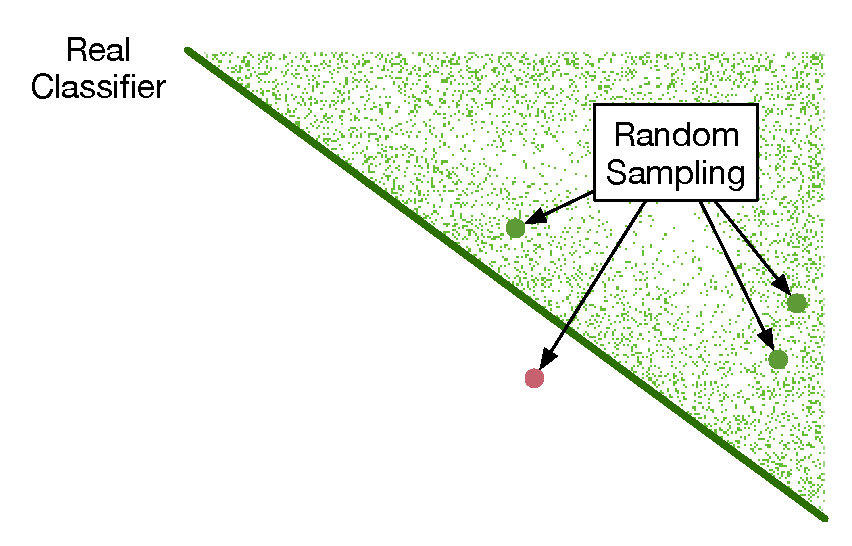
\includegraphics[scale=0.3]{figures/general-sampling-0.pdf}
        \caption{Random Sampling}
        \label{fig:sampling:random}
    \end{subfigure}
    \begin{subfigure}{0.23\textwidth}
        \centering
        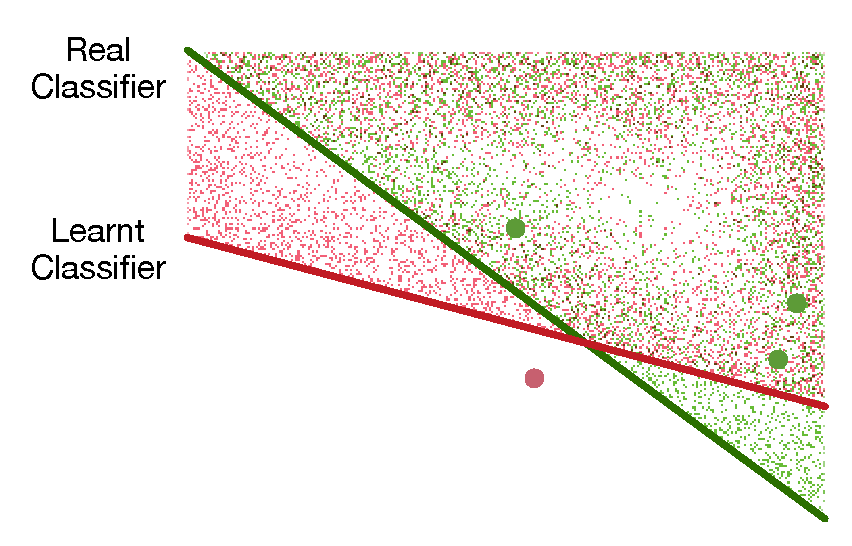
\includegraphics[scale=0.3]{figures/general-sampling-1.pdf}
        \caption{Learnt Invariant}
        \label{fig:sampling:random:invariant}
    \end{subfigure}
    \begin{subfigure}{0.23\textwidth}
        \centering
        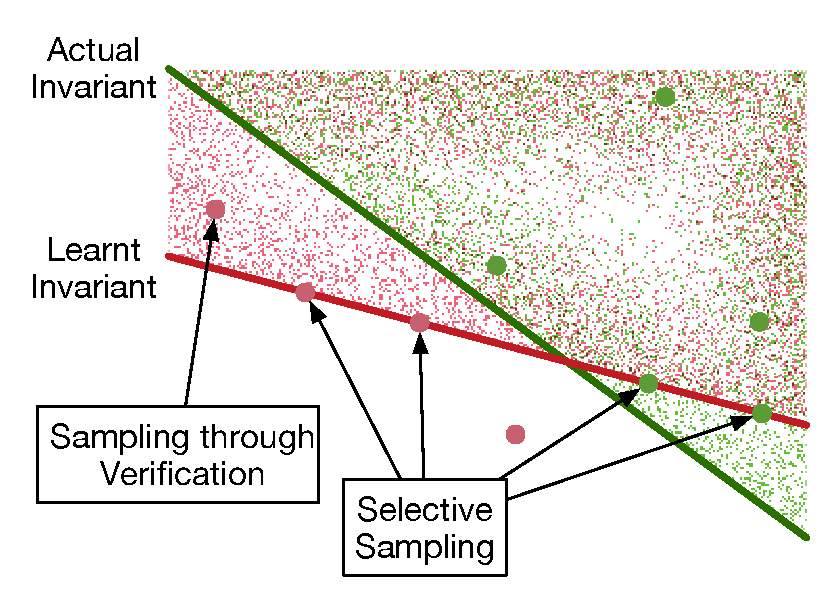
\includegraphics[scale=0.3]{figures/general-sampling-2.pdf}
        \caption{Selective and Counter-Example Sampling}
        \label{fig:sampling:selective}
    \end{subfigure}
    \begin{subfigure}{0.23\textwidth}
        \centering
        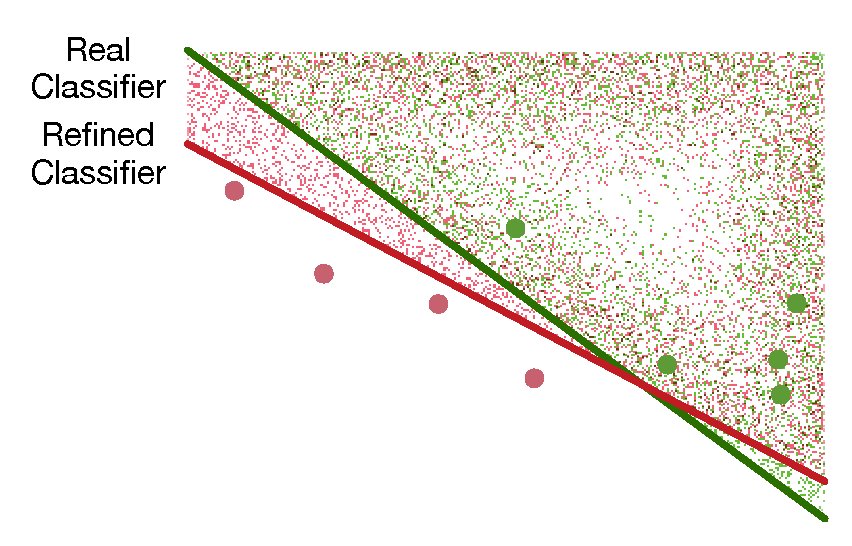
\includegraphics[scale=0.3]{figures/general-sampling-3.pdf}
        \caption{Refined Invariant}
        \label{fig:sampling:selective:invariant}
    \end{subfigure}
    \caption{Sampling Approaches}
    \label{fig:sampling}
\end{figure}

\medskip\noindent
\textbf{Random Sampling.}
Random sampling acts as an initialization sampling method 
as well as a supplementary sampling method in our framework. 
Firstly, before any invariant is learnt in our framework, 
we adopt simple random sampling solely to learn the initial invariant, 
which can be refined later in the invariant inference process. 
Secondly, the efficiency of other sampling methods, introduced in the following, 
is largely based on the similarity of the invariant candidate and the correct invariant. 
However, if the invariant candidate is very different from the correct invariant, 
random sampling can make the invariant converge faster than other sampling methods. 
Thirdly, since selective sampling can introduce biased samples distribution, 
random sampling aims at reducing its impact that can lead to a biased invariant result. 
As a result, the random sampling is applied to all the invariant inference iterations 
rather than only the first iteration. 

\medskip\noindent
\textbf{Selective Sampling.}
Selective sampling is a technique in active learning, which can generate samples which are more informative and instructive.
It is an aggressive sampling technique that helps $\textsc{Zilu}$ to learn the target much faster.

%When we have a guess of loop invariants, we can apply selective sampling approach to finding more useful samples.
%Actually we apply this sampling method all along the learning procedure except the first iteration.
It is obvious that, due to the limited set of samples we have (which is often referred to as labeled samples in the machine learning community), 
the guessed classifier obtained from previous iteration might be far from being correct. 
In fact, without labeled samples which are right on the boundary of the `actual' classifier, 
it is very unlikely that we would find it. 
Intuitively and intelligently, in order to get the `actual' classifier, 
we would require samples which would distinguish the actual one from any nearby one, 
This problem has been discussed and addressed in machine learning using active learning and selective sampling~\cite{DBLP:conf/icml/SchohnC00}.

The concept of active learning or selective sampling refers to the approaches 
that aim at reducing the labeling effort by selecting only the most informative samples to be labeled. 
SVM(supported vector machines) selective sampling techniques have been proven effective in achieving a high accuracy 
with fewer examples in many applications~\cite{DBLP:conf/mm/TongC01,DBLP:journals/jmlr/TongK01}. 
The basic idea of selective sampling is that at each round, we select the samples that are the closest to the classification boundary 
so that they are the most difficult to classify and the most informative to label. 
Since an SVM classification function is represented by support vectors which are the samples closest to the boundary, 
this selective sampling effectively learns an accurate function with fewer labeled data~\cite{DBLP:conf/icml/SchohnC00}. 
In our setting, this means that we should sample a program state right by the classifier and test the program 
with that state to label that feature vector so that the classifier would be improved.


%Algorithm~\ref{alg:active} presents details on how active learning is implemented in \textsc{Zilu}. 
%At line 2, we obtain a classifier based on Algorithm~\ref{classify}. 
%We compare the newly obtained classifier with the previous one at line 4, if they are identical, we return the classifier; 
%otherwise we apply selective sampling so that we can generate additional labeled samples for improving the classifier. 
%In particular, at line 5, we apply standard techniques~\cite{DBLP:conf/icml/SchohnC00} to select the most informative sample. 
%Notice that in our setting, the most informative samples are those which are exactly on the lines and 
%therefore can be obtained by solving an equation system. 
%At line 8, we test the program with the newly generated samples so as to label them accordingly.
After the above discussion, apparently the pre-requirement of selective sampling is there is a guess.
Thus in our implementation, after learning an invariant candidate, 
which is usually a single polynomials or conjunction or disjunction of polynomials,
we do sample along this or these polynomials by using \textbf{GSL}~\cite{gough2009gnu} to solve them.

This technique is applied all along the learning process except the very beginning.

\medskip\noindent
\textbf{Counter-Example Sampling.}
Compared with the above sampling techniques, we should admit counter-example sampling is more directly and objective.  
Having an invariant candidate, $\textsc{Zilu}$ tries to valid it using symbolic execution~\cite{king1976symbolic}\cite{khurshid2003generalized}
(or known as concolic testing~\cite{sen2007concolic}) and constraint solving,
which is shown in detail in Section ~\ref{sec:verification}.
If it fails to validate, the constraint solver could provide us with counter-examples that can directly refute our invariant candidate.
And as a result, it is quite useful for the invariant candidate refinement in the next learning procedure.

As counter-example sampling technique sounds good, it seems this technique should be applied almost all the time, 
but the fact is it is applied only after failure of invariant candidate verification.
That is because applying concolic testing and constraint solving is a more time-consuming job than the other two sampling methods.

% subsection sampling_approaches (end)

\subsection {Labeling}
\label{subsec:labeling}
With the sample set $S$ from the last step, we test the program starting with each program state $s$ in $S$. 
As said in the introduction part, $Body(s)$ is the state which could be reached after executing $Body$ from state $s$.
We write $Body^*(s)$ to denote the set of program states which could be reached after executing zero or more iterations of the loop starting from $s$.
Furthermore, we write $s \Rightarrow\Rightarrow s'$ to denote that starting with a program state $s$ would result in state $s'$ when the loop terminates. 

So if there is a trace $Trace\{s_0 \to s_1 \to ...\to s_i \to ... \to s_n\}$, 
where $s_0$ is the initial state before entering the loop, 
$s_i$ is a state just after the loop has ran $i$ iteration in the program,
and $s_n$ satisfies $\neg B$ and thus it is the state that can jump out the loop body,
then 
\begin{itemize}
\item $s_{i+1} = Body(s_i)\ \forall i \in [0, \ldots, n-1]$.
\item $s_{i} \in Body^*(s_0)\ \forall i \in [0, \ldots, n]$.
\item $s_{0} \Rightarrow\Rightarrow s_{n}$.
\end{itemize}
%We write $Body^*(S)$ to denote $\{s' | \exists s \in S \cdot s' \in Body^*(s)\}$. 



\subsubsection{Positive State, Negative State, Implication Pair}
\label{subsec:state}
These three concepts are previously introduced in \cite{sharma2014invariant}.
In this paper, we use predicates and sets of states interchangeably.
Let $\mathcal{C}$ be a candidate invariant.

From constraint~\ref{inv:pre} we know, for an invariant $Inv$, 
any state that satisfies $Pre$ also satisfies $Inv$. 
We call any state that must be satisfied by an actual invariant a positive state. 


Now consider constraint~\ref{inv:loop}.
This is called inductive property, which means if there is a pair of states $(s, t)$ in which $t = Body(s)$, 
and $s$ satisfies $Cond$, then $(s \models Inv) \Rightarrow (t \models {Inv})$. 
Hence, for the invariant candidate $\mathcal{C}$, 
if a pair of states $(s, t)$ in which $t = Body(s)$ satisfying $(s \models \mathcal{C}) \wedge (t \models \neg \mathcal{C})$ proves $\mathcal{C}$ is not an invariant. 
We call this pair of states as implication pair.

Finally, consider constraint~\ref{inv:post}.
The `existence of a state $s \models \mathcal{C} \wedge \neg B \wedge \neg Post$ proves $\mathcal{C}$ is inadequate to discharge the postcondition. 
We call a state $s$ which satisfies $\neg{B} \wedge \neg{Post}$ a negative state. 



\subsubsection{Positive Trace, Negative Trace, Implication Trace}
\label{subsec:trace}
For a trace $Trace\{s_0 \to s_1 \to ... \to s_i \to ... \to s_n\}$, 
if $s_0$ satisfies $Pre$, and $s_n$ satisfies $Post$,
then this is a positive trace, meaning $\forall s_i \models Inv$.
Because if state $s_0$ satisfy $Pre$,
$s_0$ is a positive state that must satisfy $Inv$, according to equation 1.
Furthermore, according to equation 2,
all of $Trace\{s_0 \to s_1 \to ...\to s_i, ... \to s_n\}$ are positive states.
So now we can get a positive trace  $Trace\{s_0 \to s_1 \to ...\to s_i \to ... \to s_n\}$.

On the contrary, for a trace $Trace\{s_0 \to s_1 \to ...\to s_i \to ... \to s_n\}$, 
if $s_0$ satisfies $\neg Pre$, and $s_n$ satisfies $\neg Post$,
we can infer this is a negative trace, 
which means all the states in this trace should be negative states.  

Actually for an arbitrary trace, there are also two other possibilities we have not mentioned yet.

One is a trace that begins with a state $s_0$ satisfying $Pre$ and ends with a state $s_n$ that satisfying $\neg Post$,
obviously, this is a counter-example to disprove the program,
which means there is something wrong with the program specification.
So if $\textsc{Zilu}$ meets any counter-example trace, 
it exits immediately with the message to tell the failure of program specification. 

The other case is a trace begin with a state $s_0$ satisfying $\neg Pre$ but ends with a state $s_n$ satisfying $Post$.
Under this condition, we could not know whether $s_0$ and $s_n$ satisfy invariants or not,
not to mention other states $\{s_1, s_2, ..., s_{n-1}\}$.
Then we name this trace as an implication trace, meaning if $s_i \models Inv$, then $s_j \models Inv$ $\forall j \ge i$.
Implication traces can not be used to do classification directly, 
however, they have strength in validating a candidate.
For instance, $\mathcal{C} = x - y \ge 0$ and there is an implication trace 
$Trace\{s_0 \to s_1 \to s_2\}$ where 
$$s_0 = \big(x \mapsto 2, y \mapsto 1\big),  s_1 = \big(x \mapsto 2, y \mapsto 2\big),  s_2 = \big(x \mapsto 2, y \mapsto 3\big).$$
After using $\mathcal{C}$ to label this trace, we find out $$s_0 \mapsto +,  s_1 \mapsto +,  s_2 \mapsto -$$ 
violates the above trace $Trace\{s_0 \to s_1 \to s_2\}$ which means the current $\mathcal{C}$ is not an actual invariant.
In this case, $\textsc{Zilu}$ return to sampling stage to get more data for learning.
%In total, we can have table.~\ref{LabelingTable}.


So now we categorize all the program states $Body^*(S)$ started from Set $S$ into four sets:
$\mathcal{S}^\chi$ which stands for counter-example trace, 
$\mathcal{S}^+$ which stands for positive traces, 
$\mathcal{S}^-$ which stands for negative traces, 
and $\mathcal{S}^\rightarrow$ which stands for implication traces.

They can be judged according to Table~\ref{tab:labeling}: 
\begin{table}[htb]
\label{tab:labeling}
\centering
\begin{tabular}[float]{|c|c|c|}
\hline
$s_0 \Rightarrow \Rightarrow s_n$ & $s_n \models Post$            & $s_n \models \neg Post$\\
\hline
$s_o \models Pre$                 & $Body^*(s_0) \in \mathcal{S}^+$       & $Body^*(s_0) \in \mathcal{S}^\chi$\\
\hline
$s_0 \models \neg Pre$            & $Body^*(s_0) \in \mathcal{S}^\rightarrow$       & $Body^*(s_0) \in \mathcal{S}^-$\\
\hline
\end{tabular}
\caption{Trace Labeling Table}
\end{table}

% section sampling (end)
